\documentclass[11.5pt]{sig-alternate} % sets document style to sig-alternate
% packages
% typesetting
%\usepackage{dirtytalk} % typset quotations easier (\say{stuff})
\usepackage{hanging} % hanging paragraphs
\usepackage[defaultlines=3,all]{nowidow} % avoid widows
\usepackage[pdfpagelabels=false]{hyperref} % produce hypertext links, includes backref and nameref
\usepackage{xurl} % defines url linebreaks, loads url package
\usepackage{microtype}
%\usepackage{textcomp}
%\newcommand{\texttildemid}{\raisebox{0.4ex}{\texttildelow}}
% layout
\usepackage{enumitem} % control layout of itemize, enumerate, description
\usepackage{fancyhdr} % control page headers and footers
\usepackage{float} % improved interface for floating objects
%\usepackage{multicol} % intermix single and multiple column pages
% language
\usepackage[utf8]{inputenc} % accept different input encodings
\usepackage[english]{babel} % multilanguage support
% misc
\usepackage{graphicx} % builds upon graphics package, \includegraphics
%\usepackage{lastpage} % reference number of pages
%\usepackage{comment} % exclude portions of text (?)
\usepackage{xcolor} % color extensions
\usepackage[backend=biber, style=apa]{biblatex} % sophisticated bibliographies % necessary for HTML to display author info and date on abstract page
\usepackage{csquotes} % advanced quotations, makes biblatex happy
\usepackage{authblk} % support for footnote style author/affiliation
% tables and figures
\usepackage{tabularray}
%\usepackage{array} % extend array and tabular environments
\usepackage{caption} % customize captions in figures and tables (rotating captions, sideways captions, etc)
%\usepackage{cuted} % allow mixing of \onecolumn and \twocolumn on same page
\usepackage{multirow} % create tabular cells spanning multiple rows
%\usepackage{subfigure} % deprecated, support for manipulation of small figures
%\usepackage{tabularx} % extension of tabular with column designator "x", creates paragraph-like column whose width automatically expands
%\usepackage{wrapfig} % allows figures or tables to have text wrapped around them
%\usepackage{booktabs} % better rules
% dummy text
%\usepackage{blindtext} % blind text dummy text
%\usepackage{kantlipsum} % Kant style dummy text
\usepackage{lipsum} %lorem ipsum dummy text
% other helpful packages may be booktabs, longtable, longtabu, microtype

\pagestyle{fancy} % sets pagestyle to fancy for fancy headers and footers

% header and footer
% modern way to set header image
\renewcommand{\headrulewidth}{0pt} % defines thickness of line under header
\renewcommand{\footrulewidth}{0pt} % defines thickness of line above header
\setlength\headheight{80.0pt} % sets height between top margin and header image, effectively moves page contents down
\addtolength{\textheight}{-80.0pt} % seems to affect the lower height. maybe only works properly if footer numbers enabled?
\fancyhf{}
\fancyhead[CE, CO]{
\includegraphics[width=\textwidth]{headerImage.png}}
% footer
%\fancyfoot[LE,LO]{Article Title Here \\ DOI: }% left footer article title and doi
%\fancyfoot[CE,CO]{{}} % center footer empty
%\fancyfoot[RE,RO]{\thepage} % right footer page numbers
%\pagenumbering{arabic} % arabic (1, 2, 3) numbering in footer

\hypersetup{colorlinks=true,urlcolor=blue} % sets link color to blue
\urlstyle{same} % sets url typeface to same as rest of text

% set caption and figure to italics, label bold, left align captions, does not transfer to HTML
\captionsetup{labelfont=bf, font={large, it}, justification=raggedright, singlelinecheck=false}
\renewcommand\theContinuedFloat{\alph{ContinuedFloat}}

%this next bit is confusing, but essentially changes the width of the abstract. Seems to have been copied from this https://tex.stackexchange.com/questions/151583/how-to-adjust-the-width-of-abstract
\let\oldabstract\abstract
\let\oldendabstract\endabstract
\makeatletter %changes @ catcode to enable modification (in parsep)
\renewenvironment{abstract} %alters the abstract environment
{\renewenvironment{quotation}%
               {\list{}{\addtolength{\leftmargin}{1em} % change this value to add or remove length to the the default ?
                        \listparindent 1.5em%
                        \itemindent    \listparindent%
                        \rightmargin   \leftmargin%
                        \parsep        \z@ \@plus\p@}%
                \item\relax}%
               {\endlist}%
\oldabstract}
{\oldendabstract}
\makeatother %changes @ catcode to disable modification

% checks
% italics 
% links -
% dashes -
% tildes -
\begin{document}

\title{Stemming on STEM: A STEM Education Framework for Students with Disabilities}

\author[1]{\large \color{blue}Jiwon Hwang}
\author[2]{\large \color{blue}Jonte C. Taylor}

\affil[1]{California State University, Bakersfield}
\affil[2]{The Pennsylvania State University}

\toappear{}
%% ABSTRACT
\maketitle
\begin{@twocolumnfalse} 
\begin{abstract}
\item 
\textit{There has been increased attention paid to science, technology, engineering, and mathematics also known as STEM. The focus on STEM has been both educational and occupational. Unfortunately, students with disabilities perform below their peers without disabilities in math and science. The authors discuss issues related to STEM and students with disabilities. These issues include (1) traditional views of STEM education, (2) the importance of STEM education, and (3) students with disabilities performance in STEM. The authors posit a framework for STEM education for students with disabilities and promote the incorporation of the arts to increase students’ STEM knowledge and achievement.}
\\ \\
Keywords: STEM, science, mathematics, arts, STEAM, disabilities, education
\end{abstract}
\end{@twocolumnfalse}

%% AUTHOR INFORMATION

\textbf{*Corresponding Author, Jiwon Hwang}\\
\href{mailto: jwluv1001@gmail.com }{(jwluv1001@gmail.com)} \\
\textit{Submitted Jan 3 2016 }\\
\textit{Accepted  Apr 13 2016} \\
\textit{Published online Jun 13 2016} \\
\textit{DOI: 10.14448/jsesd.09.0003} \\
\pagebreak
\clearpage
\begin{large}
\section*{WHAT IS STEM?}

In recent years there has been increased attention paid to science, technology, engineering, and mathematics across diverse fields of research and practice, framed as the acronym “STEM”.  Although these four disciplines have been banded together under the same umbrella, there eludes consensus of the extent of their interconnectedness with some positing that they are separate knowledge bases (Bell \& Lederman, 2003; Clough, 2000) and others contending that they are bridged (Kaufman, 2003; Morrison, 2006).  Although researchers, practitioners, policy makers, curriculum developers, and others have defined STEM in various ways to adjust its use in their fields, STEM has been widely used as the generic label of a higher category spanning four areas across various fields (e.g., education, business, and events/programs) (Kuenzi, 2008; Morrison \& Raymond, 2009; Johnson, 2012).  As a result, STEM is now universally perceived as referring to one or several areas of the four disciplines. 

According to Zollman (2012), the comprehensive purposes of STEM are to address societal and personal needs to be a fulfilled citizenry.  Students who are STEM proficient prepare the nation to be a global leader in an increasingly global economy (Hughes, 2010).  In addition to the importance of STEM from a global perspective, teaching and learning STEM disciplines are also valuable in enhancing the quality of daily life for students, especially for those with disabilities.  Students who have advanced knowledge in STEM are more likely to have greater work-related opportunities (Basham \& Marino, 2010). According to the U.S. Department of Education (2015), up to 62\% of the fastest growing careers require proficient knowledge or skills in STEM-related areas (Basham \& Marino, 2013; Kaku, 2011).  Moreover, knowledge in STEM helps students to live a better quality of life because STEM is fully embedded in daily life situations (e.g., calculating tips, using electronic devices such as smartphones and iPads, and using chemicals such as shampoos and candles).

However, U.S. students tend to avoid majoring in STEM areas (Apedoe, Reynolds, Ellefson, \& Schunn, 2008; Basalyga, 2003; Lam, Doverspike, Zhao, Zhe, \& Menzemer, 2008).  According to a report from the American College Testing (ACT, 2015), although students’ interest in STEM has been slightly increased by 1\% in the recent five-year trajectory, the percentage of students’ interest in science has been continuously decreased by one percent.  Consequently, approximately 50\% of high school graduates failed to meet the college readiness benchmark (ACT, 2015).  Students tend to experience significant difficulties, particularly in mathematics and science, from elementary school through college, which continuously builds negative views of STEM. As shown in the National Report Card from 2009 to 2015, the majority of students nationwide did not successfully reach an adequate level of proficiency (e.g., 67\% and 68\% of 8th grade students were below proficient in mathematics and science, respectively).  The situation appears even more severe when performance in mathematics and science is compared internationally.  The Program for International Student Assessment (PISA, 2012), the U.S. ranked 35th in mathematics and 27th in science out of 64 countries (Organization for Economic Cooperation and Development [OECD], 2013).  The severity of the performances for students with disabilities is even greater when compared to their peers.  While comparing international scores of students with disabilities is virtually impossible due to varying definitions for determining disability, nationally, students with disabilities perform significantly lower than their peers without disabilities (Aronin \& Floyd, 2013; Basham \& Marino, 2013; National Center for Education Statistics, 2013). 

Recognizing the crisis in the U.S., there have been active movements to prepare future generations by equipping them with a higher quality of STEM education.  Recently, President Barack Obama (2009) made STEM education a priority and called for an increase in the number of students and teachers who are proficient in these fields with hopes of improving international performance.  As a result, the U.S. government allocated a large amount in federal, state, and local budgets to support teachers and students to promote proficiency in STEM disciplines and education reform, with emphasis in K-12 education.  Although research in STEM disciplines for students with disabilities is still growing, practical guidelines for teachers in inclusive and non-inclusive settings have been suggested and developed to enhance students’ success and accessibility to STEM (Basham \& Marino, 2010; Dunn, Rabren, Taylor, \& Dotson, 2012; Ludlow, 2013).

\subsection*{Educational Perspectives on STEM: Interdisciplinary Approach}

Regardless of its importance, however, “STEM” is still a buzzword in education that is ambiguous and has no clear definition or framework.  There have been numerous attempts to recognize and interpret STEM in educational perspectives.  Some researchers have referred to STEM education as a broad education category involving math, science, engineering, or technology education; thus, teaching any one of the four disciplines can simply be referred to as STEM education (Cotabish, Dailey, Robinson, \& Hughes, 2013; Watt, Therrien, Kaldenberg, \& Taylor, 2013).  Others consider STEM education to be the use of technology as a part of the instructional tools (e.g., iPad, pc) used in education (Aronin \& Floyd, 2013).  These perspectives consider STEM to be simply an acronym for grouping four disciplines without any relationship among four interwoven domains. 

However, in order to establish an educational system to promote better student performance in STEM disciplines, STEM education needs to be re-conceptualized.  Because each of the four disciplines have always been a part of educational curriculums, allocating more teaching time is not enough to break out of the current academic crisis.  Rather than referring to STEM education only as teaching one or several areas of the four disciplines, \textit{how} to teach STEM in a curriculum effectively to students needs to be embraced. In other words, STEM education should be framed as \textit{an interdisciplinary instructional approach when teaching STEM-related content}.  In this sense, teachers should not only focus on STEM content knowledge (“what you know”) but how students make good use of STEM knowledge (“what you can do with what you know”).
	
 Some studies have made efforts to define STEM education as an integrative approach and explored various ways to implement it in a curriculum. According to Sanders (2009), integrative STEM approaches are “approaches that explores teaching and learning between/among any two or more of the STEM subject areas and/or between a STEM subject and one or more other school subjects (p. 21).”  Moreover, other researchers defined STEM education as a meta-disciplinary approach or interdisciplinary approach, meaning the teaching of the separate disciplines of STEM as one cohesive entity to solve real-world problems (Breiner, Harkness, Johnson, \& Koehler, 2012; Labov, Reid, \& Yamamoto, 2010).  These points of view see the notion of STEM education as not being limited to mere integration of the four disciplines of STEM (e.g., teaching several disciplines at the same time), but the provision of students with the best practices to solve complex real-life problems with integrative thinking.  The ultimate goal of learning STEM disciplines is to build a well-integrated knowledge base that will be a benefit not only in students’ careers but also in the quality of their daily life.
	
 Reflecting the definitions and suggestions in previous research, the authors operationally define STEM education as follows: an interdisciplinary approach when (1) teaching between/among any two or more of STEM disciplines or (2) teaching any of the STEM disciplines integrated with other school subjects designed to prepare students to be equipped with the knowledge and skills to solve complex real-world problems.  The authors view STEM education as an instructional approach, so the emphasis is mainly on how to teach STEM-related content most effectively to students with disabilities.  Instead of teaching and learning STEM disciplines through isolated and de-contextualized facts (Basham, Israel, \& Maryland, 2010; Israel, Maynard, \& Williamson, 2013), this idea breaks down the solid boundary among the disciplines and recognizes them as a unitary idea (Morrison \& Raymond, 2009). 

\subsection*{Teaching Students with Disabilities Using a STEM Interdisciplinary Approach}

Recognizing that students with disabilities struggle in the STEM disciplines significantly more than their peers, promising instructional strategies and/or interventions have been developed for students with disabilities to enhance their performance in each of the STEM disciplines (e.g., Jitendra, DiPipi, \& Perron-Jones, 2002; Scheuermann, Deshler, \& Schumaker, 2009; Watt et al., 2013). Although there is a significant lack of research about STEM education for students with disabilities, researchers have started to pay attention to how meeting their special needs can fit into the design of instructional plans. Recently, \textit{Teaching Exceptional Children}, one of the most influential journals in special education, published a special issue about STEM education to explore various ways to support students with disabilities in the K-12 educational system. In the issue, Basham and Marino (2013) noted that the foundation of STEM education lies in engineering and suggested the Universal Design for Learning (UDL) as a curriculum design framework to implement STEM education for students with disabilities; Israel et al. (2013) and Kennedy and Wexler (2013) explored the connection among content literacy, reading, and STEM and offered recommendations to create a literacy-embedded STEM for teachers; Aronin and Floyd (2013) incorporated technology components by using iPads and apps in teaching STEM; and, finally, Moorehead and Grillo (2013) explored instructional commonality when teaching both mathematics and science and implemented a co-teaching method to benefit students in STEM learning. All these efforts viewed STEM education as an interdisciplinary approach emphasizing active collaboration among STEM disciplines and expanded it to make a connection with other subject disciplines as well (e.g., reading, literacy). 	

\subsection*{From STEM to STEAM:  Adding the Arts to STEM for Students with Disabilities}

Considering students’ frustration from unpleasant and/or unsuccessful experiences in STEM disciplines, some researchers suggested students’ motivation in learning STEM disciplines needs to be additionally considered within the interdisciplinary framework (Daugherty, 2013; Platz, 2007; Yakman, 2010). They argued that STEM education should be expanded to embrace and integrate with the disciplines of the arts in order to facilitate and promote accessibility of STEM learning. The arts include the areas of performing arts (i.e. dance, music, and theatre), presenting arts (i.e. visual arts), and producing arts (i.e. media arts), as described by the National Council for Core Arts Standards (2014). From this perspective, we believe STEM + ‘A’ (STEAM) should benefit students with disabilities as follows.
	
First, using instructional components from the arts can stimulate students’ motivation in pursuing difficult topics in STEM disciplines. As opposed to disciplines that require students to achieve a certain level at a certain time, the nature of the arts is relatively liberal and focuses more on creativity than getting a standardized correct answer, and they are often considered as an arena for self-expression. Thus, integrating the arts can lower the threshold of learning STEM disciplines because it facilitates student access to STEM knowledge. For example, teaching and learning the concept of fractions is difficult because students need to understand the relationship between two numbers above and below a short horizontal line (i.e., numerator and denominator); that the intuitive understanding of whole numbers does not hold true in fractions makes it even more difficult. In order to help students with disabilities who have nearly given up on learning this complex notion, teachers can bring musical components into a mathematics classroom. Instead of teaching a complex array of fraction concepts, engage students in musical activities such as playing drums with various beats (e.g., ½ and ¾). Students will become familiar with fractions-related concepts inadvertently throughout this type of activity, then teachers can make a connection to mathematics by explaining how to express the beats that were played in the most simple and convenient way.  As another example, connecting science instruction to the concept maps and graphic organizers as a visual support can be considered as visual arts.  Students allowed to create their own visual representations of science concepts allows students to be visually creative and provides teachers an opportunity to determine what students may or may not have learned.  Graphic organizers and concept maps have shown to be a successful visual tool for students with disabilities (see Figure 1 for examples of graphic organizers). 

 \begin{figure*}[th]
     \centering
     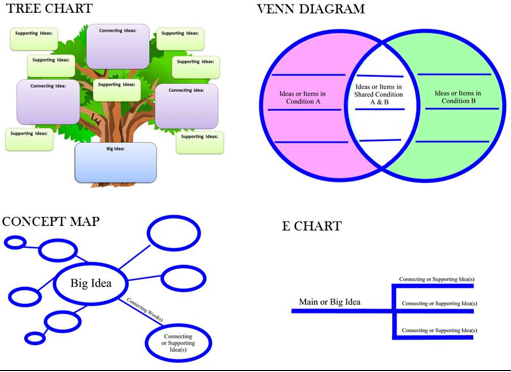
\includegraphics[width=0.9\textwidth]{fig1.png}
     \caption{ Four examples of graphic organizers as visual supports.}
 \end{figure*}

Second, the arts play critical roles as scaffolds to help students with disabilities to get into an abstract world. STEM disciplines often contain abstract concepts (Brigham, Scruggs, \& Mastropieri, 2011) that require understanding of theoretical properties beyond what students can manipulate on a practical level (Witzel, Mercer, \& Miller, 2003). Due to the poor cognitive abilities and related skills students with disabilities have been shown to have, it is important to provide scaffolds with student-participation activities that can simplify abstract concepts in order to develop precursor concepts (Devlin, 2000). Activities related to the arts can be used as a gateway to facilitate STEM learning. McGrath \& Brown (2005) suggested that the visual arts were beneficial as an instructional method for enhancing students’ learning by stimulating the higher cognitive parts of brain. Others also have also proved that manipulation of concrete objects and pictorial images remediates students’ cognitive flows and helps students’ understanding when working with abstract concepts. For example, one of the evidence-based mathematics strategies when teaching word-problem solving is the Concrete-Representational-Abstract (CRA) graduate sequence of instruction. 

The logic behind the CRA is that transforming abstract concepts into concrete and representational levels gives students sufficient opportunities to experience the concepts with visualized images and manipulatives. This should be framed within STEM education integrated with the arts. Using multimodal representations (see Figure 2) as a visual art and movement/dance as a performance art means of having students demonstrate science concepts or processes.  For example, students may be able to draw a picture of an experiment they did to explain the phenomenon of momentum or students may be able perform the process of the water cycle through movement.

\begin{table}[ht]
\begin{tabular}{|c|c|}
\hline
\multicolumn{2}{|c|}{Multimodal Representations} \\ \hline
graphs & pictures \\ \hline
data visualization & visual art \\ \hline
charts & digital art \\ \hline
writing art & diagram \\ \hline
maps & performance art \\ \hline
\end{tabular}
\captionof{figure}{List of multimodal representations for use as visual supports.}
\end{table}

\section*{CONCLUSION}

As emphasis is placed on STEM education as a means for future success, the needs of students with disabilities need to be considered.  The authors posit that by integrating the arts in STEM education, thereby transforming it to STEAM, students with disabilities are granted increased access to STEM success. As such, the authors suggest a new framework to demonstrate how STEM education should take place in a special education classroom setting (see Figure 3). The comprehensive goals are to (1) teach problem-solving skills within science contexts (e.g., problem stories about the velocity of a car, body temperatures, probability genetics, chemicals), (2) generalize problem-solving skills when engaging in hands-on activities in an engineering classroom (e.g., making a skateboard by measuring and calculating), (3) increase student motivation by integrating art and music components into a lesson to facilitate the problem-solving process (e.g., sketching pictorial images, frequency and pitch of sound), (4) promote flexibility in using various types of technology whenever needed (e.g., iPads, apps, calculators, PowerPoint), and, ultimately, (5) always make a connection to the real world. The problem-solving process within the framework the authors propose provides a practical basis for teachers to teach STEM in an integrative manner and also provides students with disabilities sufficient authentic experiences. The authors expect students with disabilities to be equipped with content knowledge and skills to solve complex problems in the real world. 

 \begin{figure}[thbp]
     \centering
     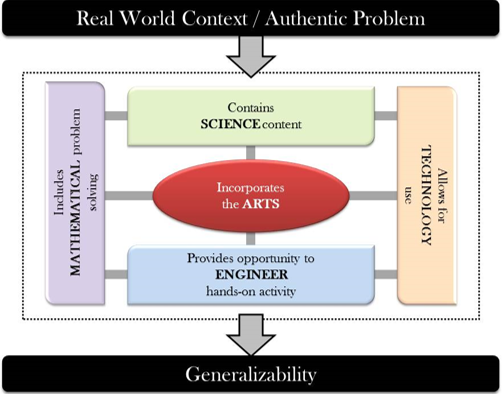
\includegraphics[width=1\linewidth]{fig3.png}
     \caption{Conceptual framework for an interdisciplinary approach to STEAM education for students with disabilities.}
 \end{figure}

\begin{table}[h]
\begin{tabular}{|c|}
\hline
Organizations for Resources \\ \hline
National Science Teachers Association (NSTA) \\ \hline
Science Education for Students with Disabilities (SESD) \\ \hline
Council for Exceptional Children (CEC) \\ \hline
CEC - Division of the Arts (DARTS) \\ \hline
Council for Children with Behavior Disorders (CCBD) \\ \hline
CEC - Division on Autism and Developmental Disabilities (DADD) \\ \hline
Association for the Gifted (TAG) \\ \hline
CEC - Division on Visual Impairments and Deaf/Blindness (DVIDB) \\ \hline
CEC - Division for Communicative Disabilities and Deafness (DCDD) \\ \hline
CEC - Division for Culturally and Linguistically Diverse Exceptional Learners (DDEL) \\ \hline
CEC - Division for Early Childhood (DEC) \\ \hline
CEC - Division for Learning Disabilities (DLD) \\ \hline
CEC - Division for Physical, Health, and Multiple Disabilities (DPHMD) \\ \hline
National Council for Teachers of Mathematics \\ \hline
The Kennedy Center ArtsEdge \\ \hline
\end{tabular}
\captionof{figure}{List of organizations and groups that focus on students with disabilities or components of STEAM.}
\end{table}

\section*{ACKNOWLEDGEMENTS}
The authors have included a list of organizations and groups that focus supports on one or more of the following areas: science, mathematics, the arts, or students with disabilities (see Figure 4).

\end{large}
\clearpage
\section*{REFERENCES}\par 

\leftskip 0.25in
\parindent -0.25in 
American College Testing (2015). \textit{The condition of college \& career readiness}. Retrieved from \url{http://www.act.org/research/policymakers/cccr13/stem.html}

Apedoe, X. S., Reynolds, B., Ellefson, M. R., \& Schunn, C. D. (2008). Bringing engineering design into high school science classrooms: The heating/cooling unit. \textit{Journal of science education and technology, 17}(5), 454–465. 

Aronin, S., \& Floyd, K. K. (2013). Using an iPad in inclusive preschool classrooms to introduce STEM concepts. \textit{Teaching Exceptional Children, 45}(4), 34-39.

Basalyga, S. (2003). Student interest in engineering is on decline. \textit{Daily Journal of Commerce}. Retrieved from \url{http://findarticles.com/p/articles/mi_ qn4184/is_20030611/ai_n1004581/}

Basham, J. D., Israel, M., \& Maynard, K. (2010). An ecological model of STEM education: Operationalizing STEM for all. \textit{Journal of Special Education Technology, 25}(3), 9.

Basham, J. D., \& Marino, M. T. (2013). Understanding STEM education and supporting students through universal design for learning. \textit{Teaching Exceptional Children, 45}(4), 8-15.

Basham, J. D., \& Marino, M. T. (2010). Introduction to the topical issue: Shaping STEM education for all students. \textit{Journal of Special Education Technology, 25}(3), 1.

Becker, K., \& Park, K. (2011). Effects of integrative approaches among science, technology, engineering, and mathematics (STEM) subjects on students' learning: A preliminary meta-analysis. \textit{Journal of STEM Education: Innovations and Research, 12}(5/6), 23.

Bell, R. L., \& Lederman, N. G. (2003). Understandings of the nature of science 	and decision 	making on science and technology based issues. \textit{Science 	Education, 87}(3), 352-377.

Breiner, J. M., Harkness, S. S., Johnson, C. C., \& Koehler, C. M. (2012). What is STEM? A discussion about conceptions of STEM in education and partnerships. \textit{School Science and Mathematics, 112}(1), 3-11

Brigham, F. J., Scruggs, T. E., \& Mastropieri, M. A. (2011). Science education and students with learning disabilities. \textit{Learning Disabilities Research \& Practice, 26}(4), 223-232.

Clough, M. P. (2000). The nature of science: Understanding how the game of science is played. \textit{The Clearing House: A Journal of Educational Strategies, Issues and Ideas, 74}(1), 13-17.

Cotabish, A., Dailey, D., Robinson, A., \& Hughes, G. (2013). The effects of a STEM intervention on elementary students' science knowledge and skills. \textit{School Science and Mathematics, 113}(5), 215-226.

Daugherty, M. K. (2013). The Prospect of an" A" in STEM Education. \textit{Journal of STEM Education: Innovations and Research, 14}(2), 10.

Devlin, K. (2000). \textit{The language of mathematics: Making the invisible visible}. New York, NY: Henry Holt and Company.

Dunn, C., Rabren, K. S., Taylor, S. L., \& Dotson, C. K. (2012). Assisting students with high-incidence disabilities to pursue careers in science, technology, engineering, and mathematics. \textit{Intervention in School and Clinic, 48}(1), 47-54.

Hughes, B. (2010). Park Forest Middle School STEM Education Fair 2010. \textit{Technology and Engineering Teacher, 70}(2), 32-35.

Israel, M., Maynard, K., \& Williamson, P. (2013). Promoting literacy-embedded, authentic STEM instruction for students with disabilities and other struggling learners. \textit{Teaching Exceptional Children, 45}(4), 18-25.

Jitendra, A., DiPipi, C. M., \& Perron-Jones, N. (2002). An exploratory study of schema-based word- problem-solving instruction for middle school students with learning disabilities: An emphasis on conceptual and procedural understanding. \textit{The Journal of Special Education, 36}(1), 23–38. doi:10.1177/00224669020360010301

Johnson, C. C. (2012). Implementation of STEM education policy: Challenges, progress, and lessons learned. \textit{School Science and Mathematics, 112}(1), 45-55.

Kaku, M. (2012). \textit{Physics of the future: How science will shape human destiny and our daily lives by the year 2100}. New York, NY: Anchor.

Kaufman, D., Moss, D., \& Osborn, T. (2003). \textit{Beyond the boundaries: A trans-disciplinary approach to learning and teaching}. Praeger, Westport, Connecticut:

Kennedy, M. J., \& Wexler, J. (2013). Helping Students Succeed within Secondary-Level STEM Content Using the “T” in STEM to Improve Literacy Skills. \textit{Teaching Exceptional Children, 45}(4), 26-33.

Kuenzi, J. (2008, March 21). Science, Technology, Engineering, and Mathematics (STEM) Education: Background, Federal Policy, and Legislative Action. Retrieved from \url{http://digitalcommons.unl.edu/crsdocs/35}

Labov, J. B., Reid, A. H., \& Yamamoto, K. R. (2010). Integrated biology and undergraduate science education: a new biology education for the twenty-first century? \textit{CBE-Life Sciences Education, 9}(1), 10-16.

Lam, P. C., Doverspike, D., Zhao, J., Zhe, J., \& Menzemer, C. C. (2008). An evaluation of a STEM program for middle school students on learning disability related IEPs.\textit{ Journal of STEM education, 9}(1/2), 21.

Ludlow, B. (2013). Growing STEM as a pathway to the future. \textit{Teaching Exceptional Children, 45}(4), 4.

McGrath, M. B., \& Brown, J. R. (2005). Visual learning for science and engineering. \textit{Computer graphics and applications, IEEE, 25}(5), 56-63.

Morrison, J. S. (2006). Attributes of STEM education: The students, the academy, the classroom. \textit{Teaching Institute for Excellence in STEM (TIES) STEM Education Monograph Series}.

Morrison, J., \& Raymond, V. (2009). STEM as a Curriculum. Education Week, 23. Retrieved from \url{http://www.edweek.org/ew/section/opinion/index.html}

Moorehead, T., \& Grillo, K. (2013). Celebrating the Reality of Inclusive STEM Education Co-Teaching in Science and Mathematics. \textit{Teaching Exceptional Children, 45}(4), 50-57.

National Center for Education Statistics (2013). National assessment of educational progress (NAEP) 2011 science assessments.  Washington, D. C.: United States Department of Education.

National Coalition for Core Arts Standards (2014) National Core Arts Standards.  Dover, DE:  State Education Agency Directors of Arts Education.  Retrieved from \url{http://www.nationalartsstandards.org}. 

Obama, B. (2009). Remarks by the President on the “Education to Innovate” Campaign. Retrieved from \url{http://www.whitehouse.gov/the-press-office/remarks-president-education-innovate-campaign}

Organization for Economic Cooperation and Development (OECD). (2013). \textit{PISA 2012 Assessment and analytical framework: Mathematics, reading, science, problem solving and financial literacy}, OECD Publishing. Retrieved from http://dx.doi.org/10.1787/9789264190511-en.

Platz, J. (2007). How do you turn STEM into STEAM? Add the arts.\textit{ Columbus: Ohio Alliance for Arts Education}, 1-5.

Sanders, M. (2009). STEM, STEM education, STEM mania. \textit{Technology Teacher, 68}(4), 20–26. 

Scheuermann, A. M., Deshler, D. D., \& Schumaker, J. B. (2009). The effects of the explicit inquiry routine on the performance of students with learning disabilities on one-variable equations. \textit{Learning Disability Quarterly, 32}(2), 103–120.

Thompson, R., \& Bolin, G. (2011). Indicators of Success in STEM Majors: A Cohort Study. \textit{Journal of College Admission, 212}, 18-24.

Watt, S. J., Therrien, W. J., Kaldenberg, E., \& Taylor, J. (2013). Promoting inclusive practices in inquiry-based science classrooms. \textit{Teaching Exceptional Children, 45}(4), 40.

Witzel, B. S., Mercer, C. D., \& Miller, M. D. (2003). Teaching algebra to students with learning difficulties: An investigation of an explicit instruction model. \textit{Learning Disabilities Research \& Practice, 18}(2), 121-131.

Yakman, G. (2010). STEAM: A framework for teaching across the disciplines.

Zollman, A. (2012). Learning for STEM literacy: STEM literacy for learning. \textit{School Science and Mathematics, 112}(1), 12-19.

\end{document}